\chapter{Amplifier Design}\label{ch:amp}

	After down-conversion, the signal must be amplified twice according to the chip design in \autoref{chap:sysdes}. Furthermore, the LO-signal controlling the mixer also needs amplification. The function and purpose of these three amplifiers are explained in this chapter.
	
	\section{Introduction}
		\subsection{Function}
			The purpose of an amplifier is to amplify electric signals. In a radar receiver setup the amplifier is often, after a limiter and a filter, the first element an incoming signal sees. Any degradation of the signal's power before the first amplification increases the noise (see \autoref{fig:noise_example}). The main goal of such an amplifier is to provide gain without adding noise, and is called an LNA (low noise amplifier).
			
			The last amplifier in a transmitter-setup is more focused on providing as much gain and output power as possible without consuming too much power. For most amplifiers it is also of concern to operate linearly. This is measured with $IIP3$ and $P_{1dB}$ as explained in \autoref{sec:ip3}.
			
			An amplifier designed with FET-technology needs a drain-supply voltage $v_{ds}$ (drain-source), see \autoref{fig:fet-illustrative}. The current through the FET, $i_{ds}$ (drain-source) depends on the gate-source voltage $v_{gs}$. The incoming signal, which is fed to the gate-terminal, controls the current through the FET which amplifies the signal.
			
		\begin{figure}[hbt!]
			\centering
			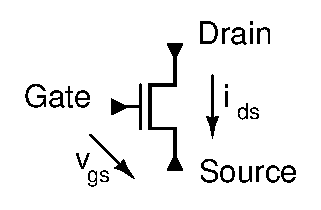
\includegraphics[width=0.3\textwidth]{fig/amplifiers/fet-illustrative}
			\caption[The ports of a FET.]{The ports of a FET. The voltage $v_{gs}$ (gate-source) controls how much current $i_{ds}$ can flow through the FET.}\label{fig:fet-illustrative}
		\end{figure}
			
		\subsection{Bias point}
			When operating the FET there are in general four different bias points corresponding to different classes of amplifiers.\autocite{gonzalez84} For example, see \autoref{fig:fet_bias_point}. For low noise operation, bias point A is common and for high output-power and class A operation, bias point C is more prevalent.
					
			\begin{figure}[hbt!]
				\centering
				\includegraphics[width=0.5\textwidth]{fig/amplifiers/fet_bias_point}
				\caption{Different bias points for a FET.}\label{fig:fet_bias_point}
			\end{figure}
			
		\subsection{Bias scheme}\label{sec:bias}
			The amplifiers in this project are biased using a self-biasing scheme according to \autoref{fig:if1bias}.\autocite{bahl03} This limits the size and complexity of the bias network as only one (positive) DC source is supplied. The PPH25 process, contrary to PH25, can handle a higher drain-source voltage $v_{ds}$ over the FET. This further simplifies the biasing as the supplied \unit[5]{V} DC voltage can be applied without the need of a resistor on the drain, given that this constitutes an appropriate bias point.

			\begin{figure}[hbt!]
				\centering
				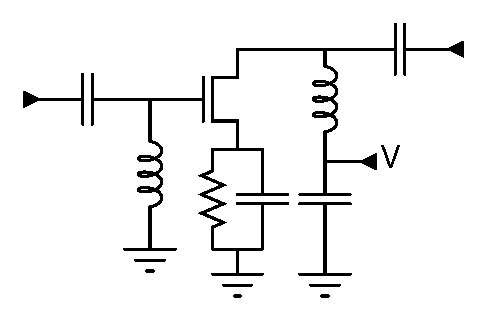
\includegraphics[width=0.5\textwidth]{fig/amplifiers/if1/bias}
				\caption[Self-bias scheme.]{The principle of the self-biasing scheme. The FET's drain is raised to $V$ and the gate is DC-grounded. The resistor on the source controls the gate-source voltage $v_{gs}$ and thereby also the bias-current $i_{ds}$.}\label{fig:if1bias}
			\end{figure}

		\subsection{Stability}
			A stable amplifier ensures that there is no oscillation.\autocite{grosch99} The amplifiers on this chip are all designed to be unconditionally stable at all frequencies. Generally an amplifier with higher gain is harder to make stable. The stability measure $K$ in \autoref{eq:kstability} is used to quantify the stability. The amplifier is unconditionally stable if $K>1$ for all frequencies.
		
			\begin{equation}\label{eq:kstability}
				K=\frac{1+|S_{11}S_{22}-S_{12}S_{21}|^2-|S_{11}|^2-|S_{22}|^2}{2|S_{12}||S_{21}|}
			\end{equation}

		\subsection{Power utilization}\label{sec:power}
			As the DC-power consumption of a amplifier increases, the linearity ($P_{1dB}$ and $IIP_3$) increases. This is evident as compression will occur at higher power (\autoref{sec:p1db}). The LO amplifier is designed to operate in compression and as such it does not benefit from high power. The remaining available DC-power is divided between the first and the second IF amplifier. As the $IIP_3$ for the second amplifier affects the system more than that of the first one, the power utility here is higher.
			
	\section{Constant power LO-amplifer}\label{sec:lo_amp}
		\subsection{Introduction}
			The system's LO-signal is specified to \unit[-5--0]{dBm} and therefore there is a need to amplify this signal. The purpose of the amplifier is to provide a high and constant input power to the mixer, not depending on fluctuations in the system's LO-signal. This is achieved by operating the amplifier in compression so that the mixer always sees the same LO. Also, by running the amplifier into compression, i.e. outputting a square-waved pulse, the mixer will switch faster between the on- and off-states, behaving more like an ideal switch. This results in a more linear mixer as explained in \autoref{sec:mixer_lodrive}.\autocite{vice03} %The LO-amplifier is matched against the mixer which is a highly reactive load.
			


		\subsection{Design}
			\subsubsection{Principle}
				When designing an LO-amplifier for a resistive FET mixer it is important to minimize reflections from the very reactive mixer-gate. However, attaining a well-matched gate is difficult.\autocite{yhland1999} At first, a bias-point is chosen, so that proper gain and compression is achieved. The dependence on frequency was considered too large and a weak feedback loop ($\unit[500]{\Omega}$) was implemented. A too strong feedback is undesirable because of the reduced gain and stability. A schematic and the actual layout of the amplifier are seen in \autoref{fig:sch_lo} and \autoref{fig:lo_layout}, respectively.

				
	The FET is self-biased by applying a voltage to the source, while having $v_{DC}=\unit[0]{V}$ on the gate (see \ref{sec:bias} \nameref{sec:bias}). This requires having an inductance to ground close to the gate.

			 
			As noise is not of much concern for the LO, it can be traded for stability, compression, ease of tuning and frequency independence. Since linearity is actually to be avoided and the amplifier never enters high-linearity bias-regions such as for class A-operation, the amplifier consumes small amounts of power, around \unit[100]{mW}.




			\begin{figure}[hbt!]
				\centering
				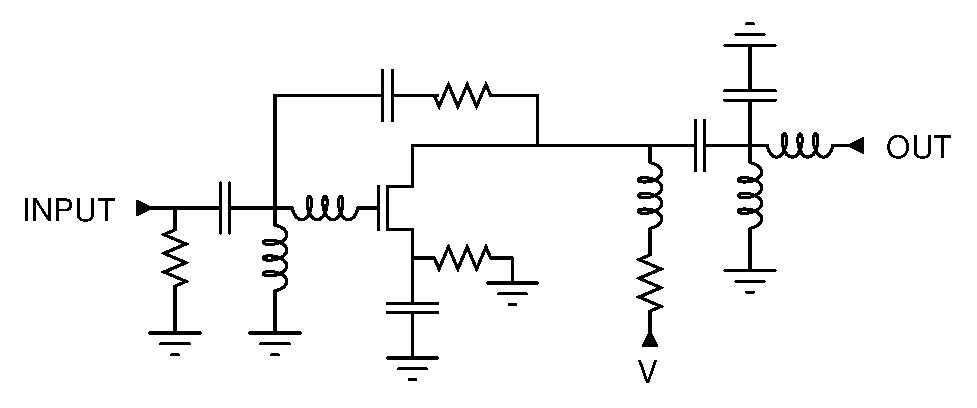
\includegraphics[width=0.85\textwidth]{fig/amplifiers/lo/sch_lo}
				\caption[LO-amplifier schematic]{Schematic of the LO-amplifier.}\label{fig:sch_lo}
			\end{figure}


			\begin{figure}[hbt!]
				\centering
				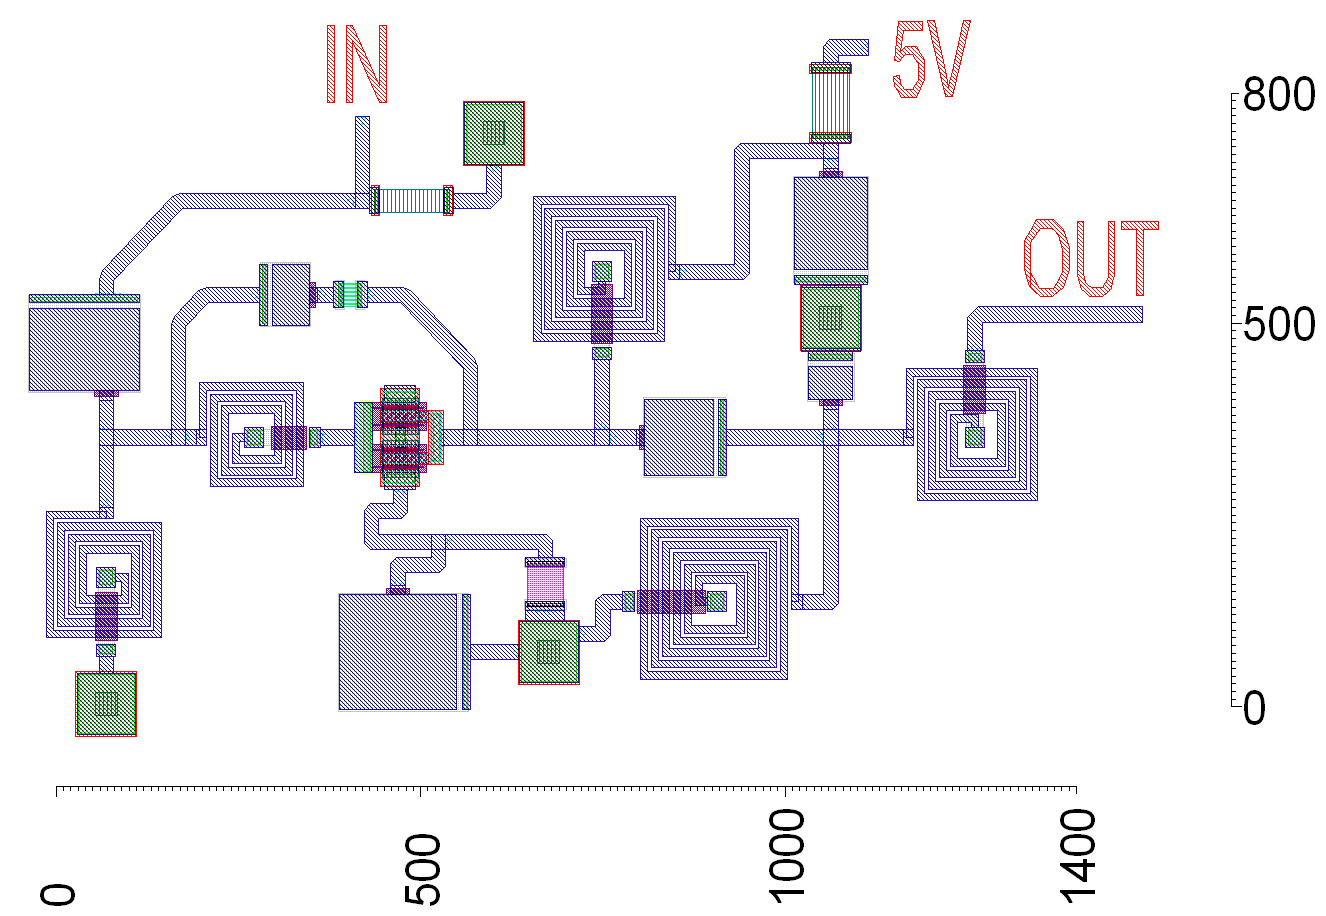
\includegraphics[width=1.0\textwidth]{fig/amplifiers/lo/layout}
				\caption[LO-amplifier layout]{The layout of the LO-amplifier with a weak parallel feedback, slightly elongated source for input matching and a self-biasing scheme.\scalemum}\label{fig:lo_layout}
			\end{figure}
			


		\subsubsection{FET-configuration and matching networks}\label{sec:lo_fet_config}
			Using large FET's results in a relatively linear operation which is to be avoided for the compression technique to work.\autocite{maas98} %, having a rather low $v_{gs}$ also means good compression.  
In \autoref{fig:FET_size_S22} the drain impedance for different FET-sizes is simulated. It shows that a smaller FET such as \unit[4$\times$25]{\mum} is a better conjugate match for the mixer since only reactive matching networks would be needed. However, such a small FET does not provide enough gain. Therefore a FET-size of \unit[4$\times$50]{\mum} is chosen. 

	The input matching network consists of an L-shaped inductor-inductor network and a shunt-resistance. The length of the source is chosen to create small input reflections. The output matching network needs to match the reactive gate of the mixing FET. This is done with a shunt capacitance and an inductance in series. The inductance to ground keeps the gate of the mixing FET at $v_{DC}=\unit[0]{V}$. 
			\begin{figure}[hbt!]
				\centering
				%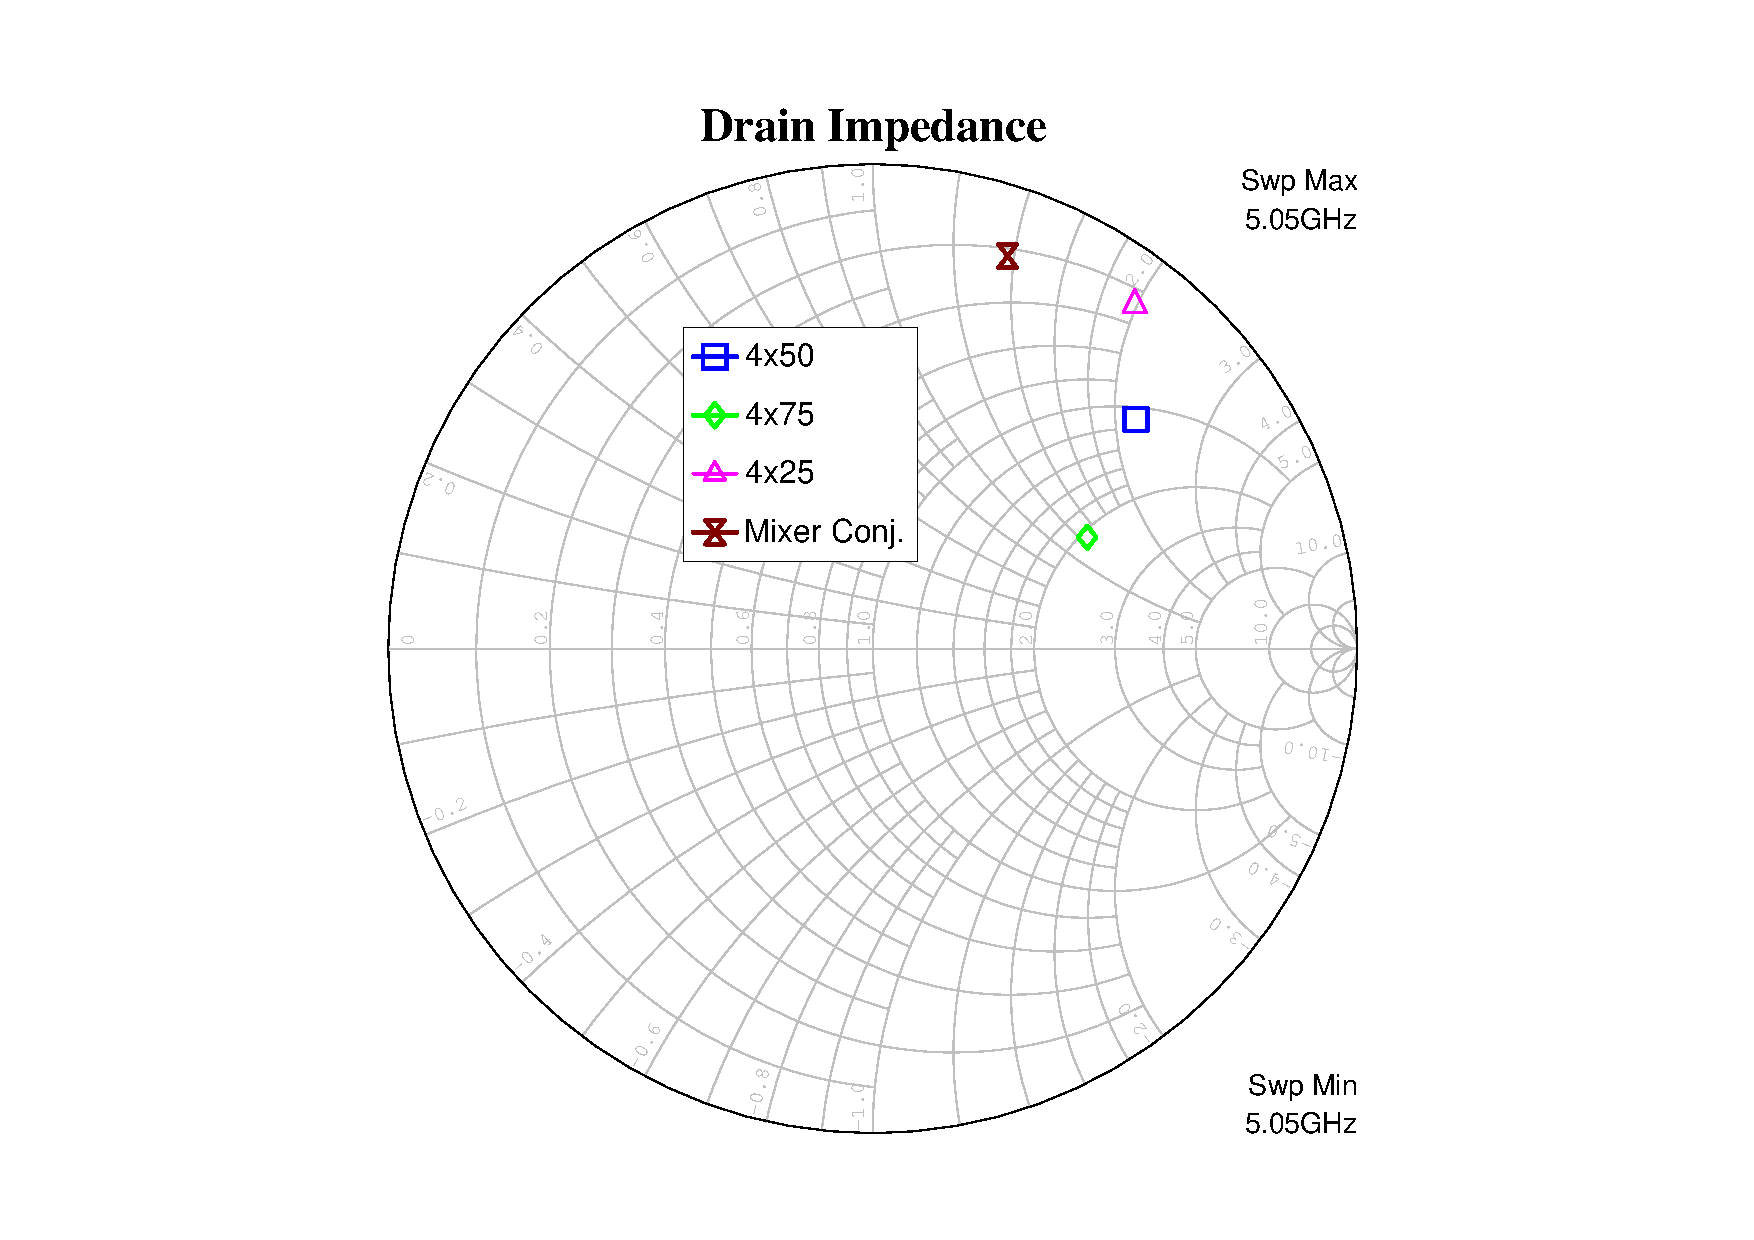
\includegraphics[trim=800 400 60 50, clip, width=0.5\textwidth]{fig/amplifiers/lo/FET_size_S22}
				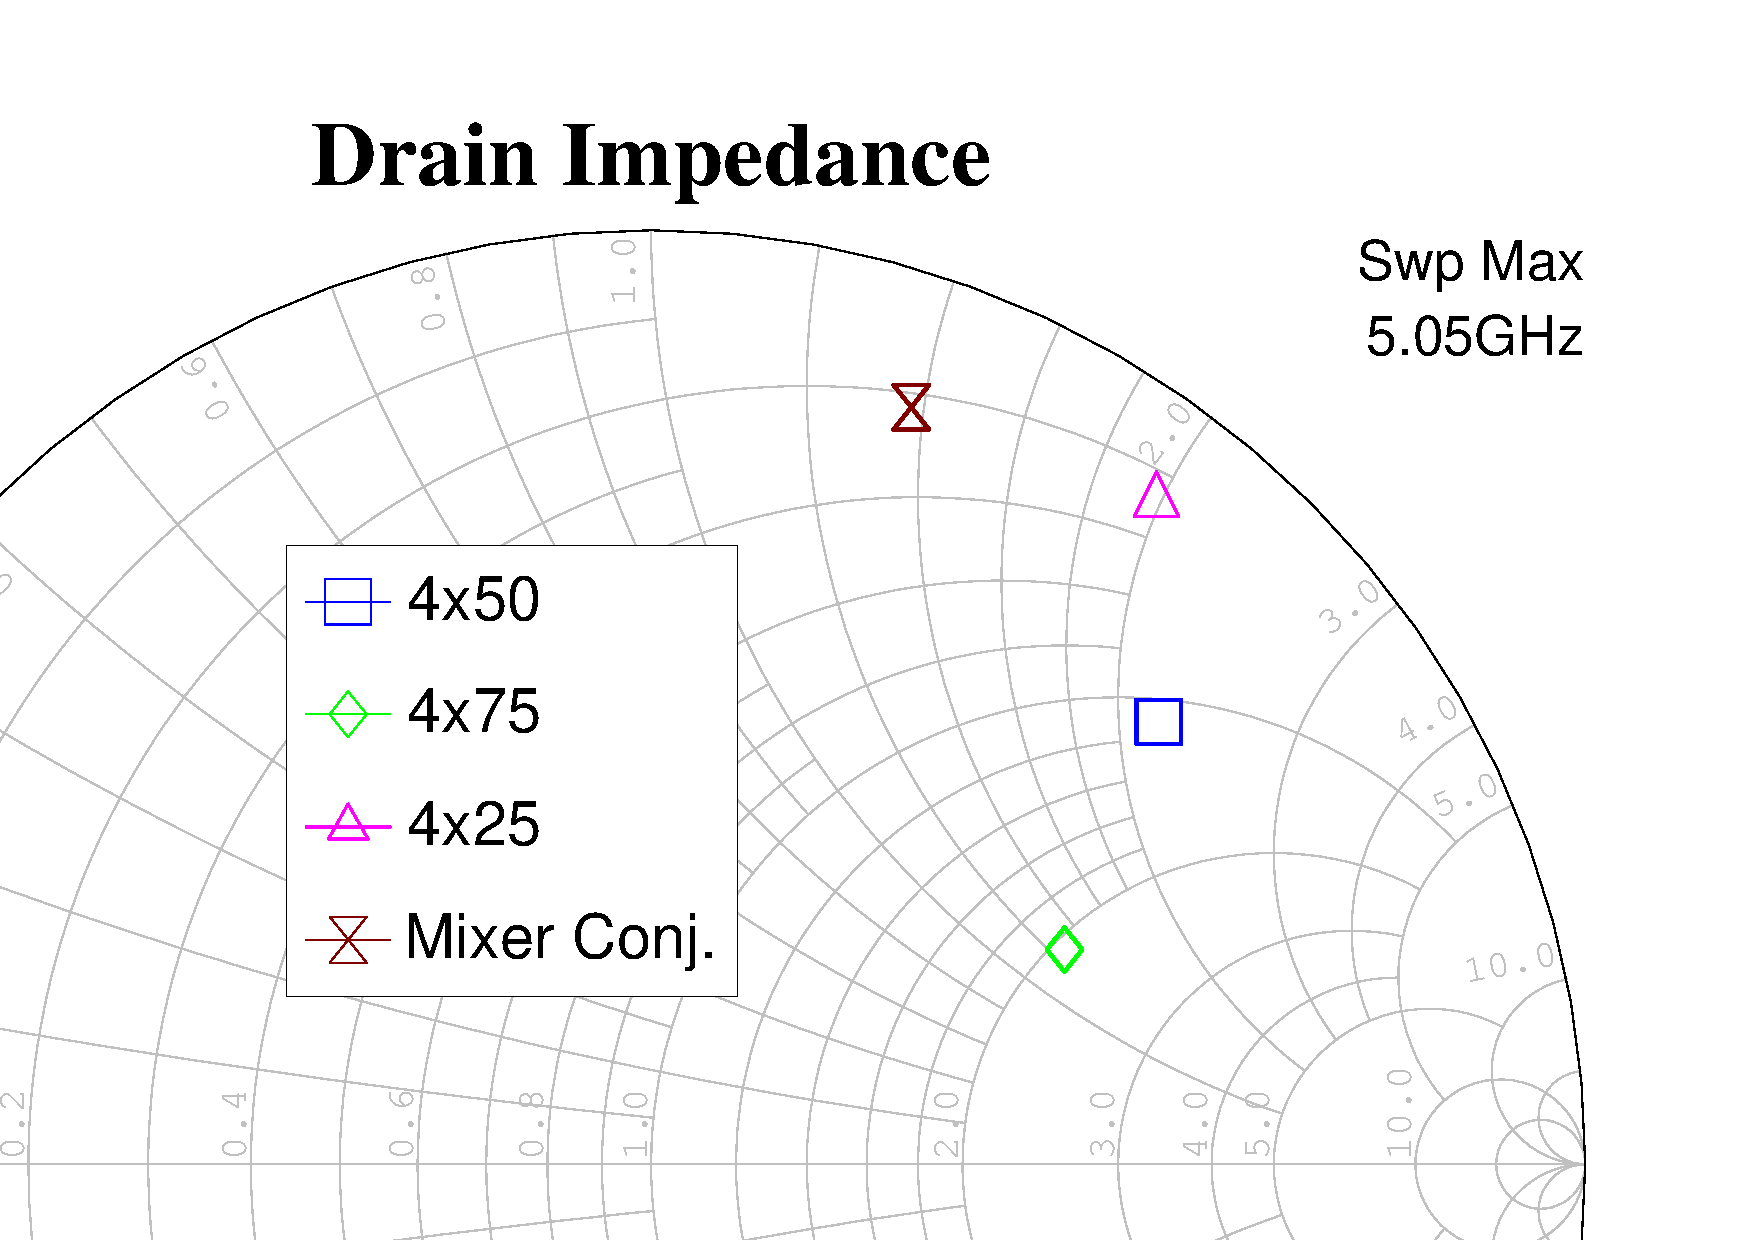
\includegraphics[width=1.0\textwidth]{fig/amplifiers/lo/FET_size_S22_zoom}
				\caption[Drain impedance for different FET's.]{The drain impedance for different FET-sizes. The \unit[4$\times$50]{\mum} and the \unit[4$\times$25]{\mum} FET-sizes make a good conjugate match for the mixer. However, \unit[4$\times$25]{\mum} does not provide enough gain.} \label{fig:FET_size_S22}
			\end{figure}

		\subsubsection{Bias point}
			The amplifier enters compression when applying a low $v_{ds}$ as seen in \autoref{fig:4x50_output_power}. The output power is shown versus input LO-power for different FET-bias points. A good bias point seems to be $v_{gs}=\unit[-0.4]{V}$, $v_{ds}=\unit[2]{V}$ which provides a signal in compression.

			\begin{figure}[hbt!]
				\centering
				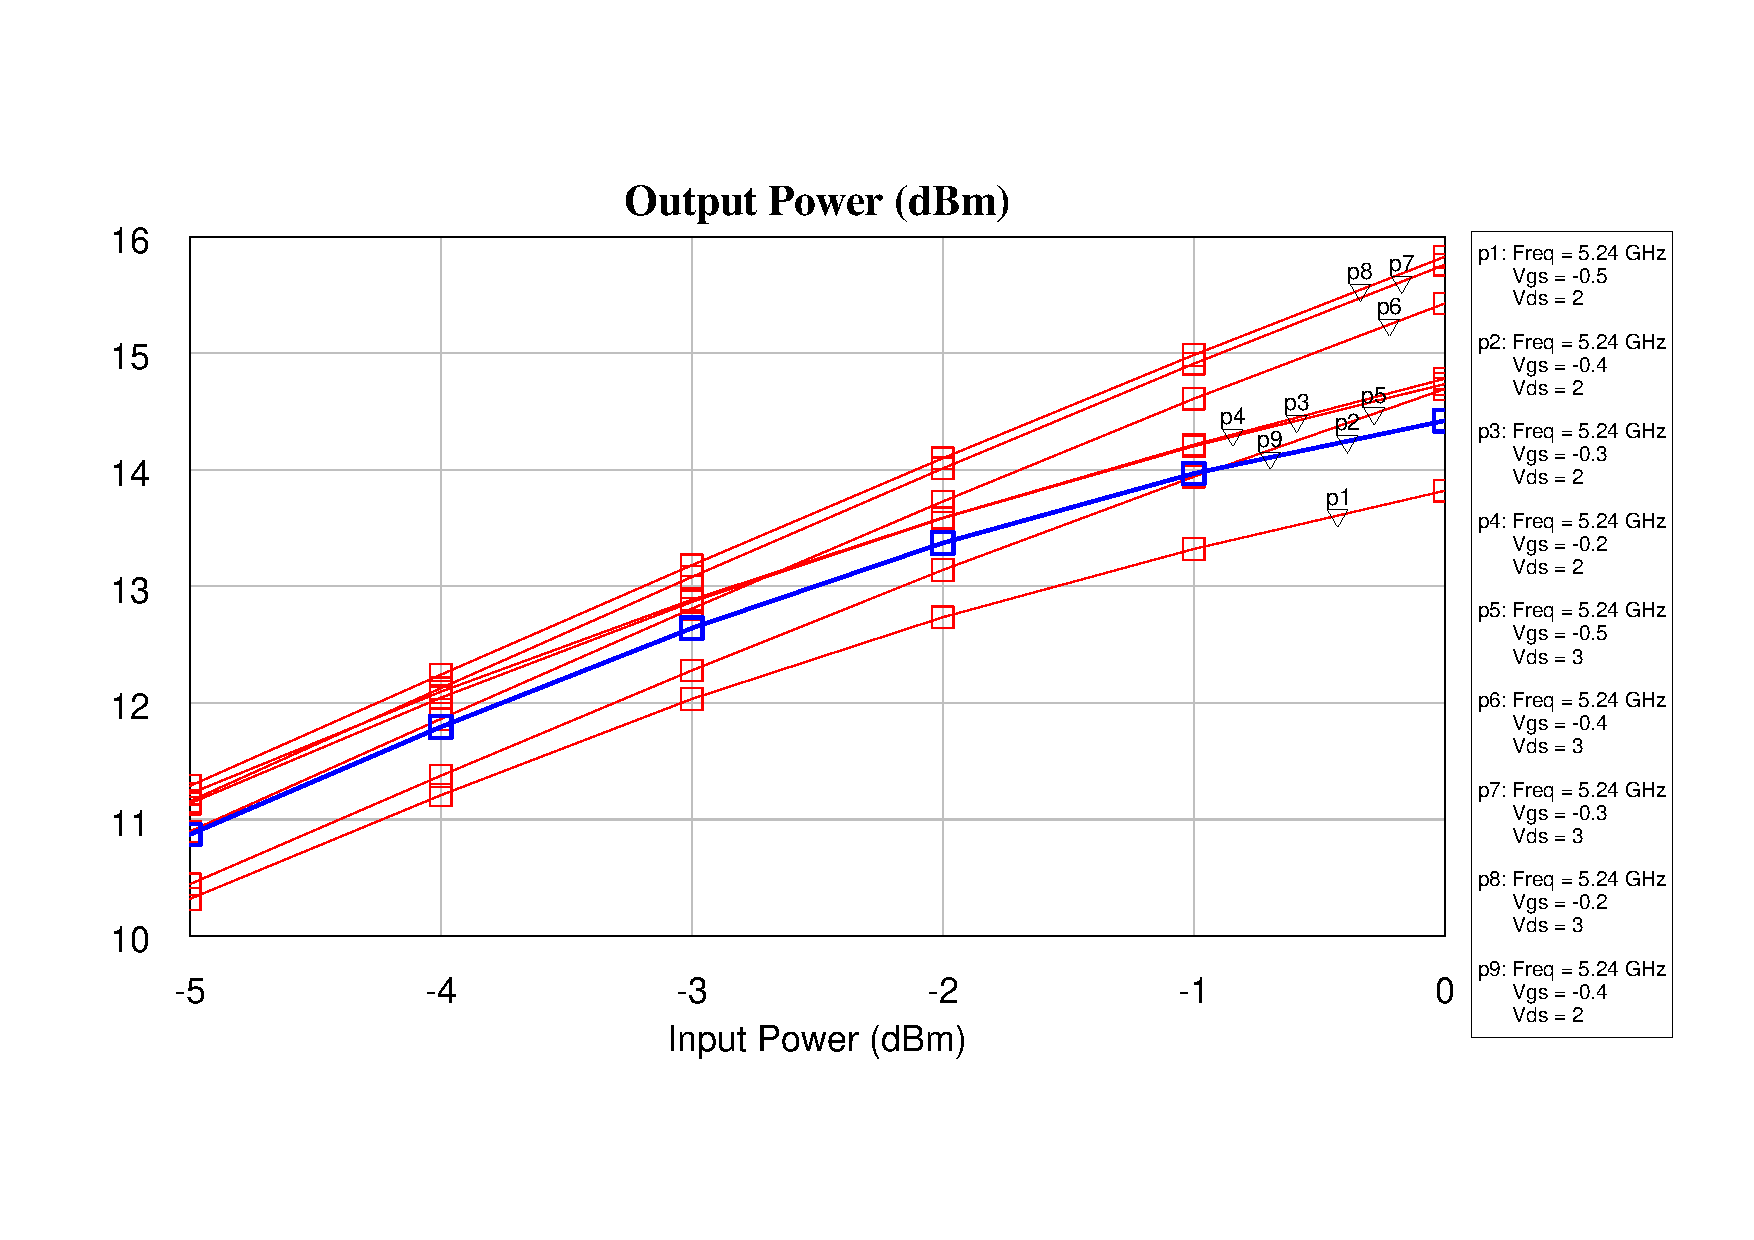
\includegraphics[trim=50 60 30 60, clip, width=0.9\textwidth]{fig/amplifiers/lo/4x50_output_power}
				\caption[Gain for different bias-points]{Output power for different bias points for the \unit[4$\times$50]{\mum} FET. The blue line represents the chosen bias-point $v_{gs}=\unit[-0.4]{V}$, $v_{ds}=\unit[2]{V}$.}\label{fig:4x50_output_power}
			\end{figure}
			





			
	%	Initially, the mixer had a matching network of it's own, tuned for \unit[50]{$\Omega$}. With this load, the main task for the LO was to maintain the high gain and compression. Later when the matching network in the mixer was fused into the LO, producing the highly reactive mixer-load \unit[12-j73]{$\Omega$}, the problem was to achieve a good match against the mixer. For the real mixer load, many elements in the matching networks could be removed, for example the series inductances on gate and drain. But the complex mixer load required all of these.
			%The impedance of the mixer was measured to \unit[$12-j73$]{$\Omega$} which the amplifier was matched against. 
		%	When changing the matching network to the reactive mixer load which basically is one big reactance, the gain drops rather drastically. However, when matched like this, the mixer doesn't require as much power. See \autoref{fig:mixerAndIdealLo} for the mixer dependence on $P_{lo}$ when matched against $Z_{lo}$.% Todo: Graf eller h
			%But the same loss would exist with a \unit[50]{$\Omega$} matched circuit, but it would be present in the mixer instead.
			
		
			

		\subsection{Simulation results}
		
			The simulation results for the LO-amplifier are presented in \autoref{tab:resultlo} for two ranges of input powers. The amplifier is operating in compression for input powers of \unit[-2--0]{dBm} and less so for weaker input powers. The power delivered into the mixing FET is shown in \autoref{fig:lo_delivered_power} and input reflections in \autoref{fig:lo_reflections}. The reflections become a problem at higher frequencies and input powers around \unit[-4]{dBm}. Good input matching is hard to achieve with the current amplifier design. As the load is changing depending on input power it is difficult to match for all input powers. Emphasis has been placed on achieving a good match for $P_{lo}=\unit[-2]{dBm}$ which is considered to be the most likely input power. The square-wave pulse is seen in figure \autoref{fig:lo_waveform}. 



%\autoref{tab:resultlo} presents LO-performance for input powers of $LO=\unit[-4$--$ -2]{dBm}$ and $LO=\unit[-2$--$0]{dBm}$. Delivered power and reflections are seen in \autoref{fig:lo_delivered_power} and \autoref{fig:lo_reflections}, respectively. The performance is good for higher input powers, for weaker input powers, the reflections become a problem at higher frequencies. Good input matching is hard to achieve with the current amplifier design. As the amplifier is running in compression, the load is changing depending on input power which makes it hard to match for all input powers. Emphasis has been placed on achieving a good match for $P_{lo}=\unit[-2]{dBm}$ which is considered to be the most likely input power. 	The square-wave pulse is seen in figure \autoref{fig:lo_waveform}.

			\begin{table}[hbt!]
				\caption[Simulation results of the LO-amplifier.]{Simulation results of the LO-amplifier.\disclaimer}
				\label{tab:resultlo}
				\centering
				\begin{tabular}{ l c c c c c c l } \toprule
					Parameter & Min. & Typ. & Max. & Min. & Typ. & Max. & Unit \\\midrule
					Frequency range & \multicolumn{3}{c}{5.04--5.54} & \multicolumn{3}{c}{5.24--5.44} & GHz \\
					Delivered Power & & & & & & \\
						\qquad @LO=\unit[-2--0]{dBm} 		& 4.0 & 4.8 & 5.5 & 4.6 & 5.0 & 5.4 & dB \\
						\qquad@LO=\unit[-4-- -2]{dBm} 		& 2.4 & 3.7 & 5.0 & 3.3 & 4.0 & 5.0 & dB \\						
					Return loss input  & & & & & & \\
						\qquad @LO=\unit[-2--0]{dBm} 	& 13.5 & 17 & & 17 & 18 & & dB \\
						\qquad @LO=\unit[-4-- -2]{dBm} 	& 10.5 & 15 & & 13 & 16 & & dB \\
					Stability $K$@\unit[0--80]{GHz} & >1 & >1 &  & >1 & >1 &  & \\
					Power consumption &  & 100 &  & & 100 & & mW  \\\bottomrule
				\end{tabular}
			\end{table}

			\begin{figure}[hbt!]
				\centering
				\includerect{0.7\textwidth}{fig/amplifiers/lo/lo_delivered_power}
				\caption[Output power from LO-amplifier]{The power delivered into the mixer from the LO-amplifier for different frequencies and LO-input powers. Measured in between amplifier and mixer. The active frequencies are 5.04 to 5.54 GHz.}\label{fig:lo_delivered_power}
			\end{figure}
			
			\begin{figure}[hbt!]
				\centering
				\includerect{0.7\textwidth}{fig/amplifiers/lo/lo_reflections}
				\caption[Input reflections of LO-amplifier]{Input reflections of LO-amplifier, weaker input-powers and higher frequencies give larger reflections. The active frequencies are 5.04 to 5.54 GHz.}\label{fig:lo_reflections}
			\end{figure}
		
			\begin{figure}[hbt!]
				\centering
				\includerect{0.7\textwidth}{fig/amplifiers/lo/lo_waveform}
				\caption[Amplifier LO waveform]{Amplifier LO running in compression, producing a square-shaped output voltage waveform.}\label{fig:lo_waveform}
			\end{figure}		
		
			
			\begin{figure}[hpt!]
				\centering 
				\subfloat[][Mixer gain when spreading LO-FET at LO=-2dBm.]{
					\includerect{0.5\textwidth}{fig/amplifiers/lo/lo_mixer_gain_spread_-2dBm}
					\label{fig:lo_mixer_gain_spread}
				} 
				\subfloat[][Mixer compression when spreading LO- and mixer-FET for LO=-2dBm.]{
					\includerect{0.5\textwidth}{fig/amplifiers/lo/lo_mixer_compression_spread_-2dBm_both_fets}
					\label{fig:lo_mixer_p1db_spread-2dBm}
				} \\
				\subfloat[][Mixer compression when spreading LO- and mixer-FET for LO=-4dBm.]{
					\includerect{0.7\textwidth}{fig/amplifiers/lo/lo_mixer_compression_spread_-4dBm_both_fets}
					\label{fig:lo_mixer_p1db_spread-4dBm}
				}			
				\caption{Conversion gain and compression point for the mixer when applying spread to the mixer- and LO-amplifier-FET. Using EM-models at $f_{rf}=\unit[3.2]{GHz}$. The observed spread in delivered LO-power is not present in \subref{fig:lo_mixer_p1db_spread-2dBm} ($P_{lo}=\unit[-2]{dBm}$) suggesting some threshold power is reached. For $P_{lo}=\unit[-4]{dBm}$, \subref{fig:lo_mixer_p1db_spread-4dBm}, the mixer's compression point is being affected by spread in the FETs.}\label{fig:lo_mixer_spread}
			\end{figure}
			
	
			
			
			%	and this is the the overtones present in the outputted signal as can be seen in the frequency spectra \autoref{fig:lo_frequency_spectra}. The effect of these on the mixer is discussed in \autoref{sec:loAndMixer}. It is common to see relatively powerful overtones like these when FET's are working near their compression point. \autocite{besser03}

		
		%	As the LO-amplifier is tuned for the mixer, the two are evaluated as one unit under \nameref{sec:mixer} in the mixer chapter. 
		
			The spread analysis, \autoref{fig:lo_spread}, suggests that the LO-amplifier is sensitive to variations. The delivered power may drop as much as \unit[2]{dB} for input powers of $\unit[-2]{dBm}$. %The frequency dependence of the spread is due to spread in the FET. 
However, when spreading the LO- and mixer-FET which seem to cause most of the spread, the mixer conversion gain and compression are hardly affected, \autoref{fig:lo_mixer_spread}. This suggests that the power supplied to the mixer is above some threshold-power where it is fair to assume that stronger LO is less important\autocite{yhland1999}. However, for $P_{LO}=\unit[-4]{dBm}$, the mixer $P_{1dB}$ is being affected, it drops on one occasion to \unit[9.7]{dBm}.

			
				%The spread in power is likely to yield the same spread in the mixer's $P_{1dB}$-point as these are linearly correlated. The mixer's conversion gain due to spread in LO is only \unit[0.2]{dB} at an input LO of \unit[-2]{dBm}. 
			
	\subsection{Gain versus compression}
		It is possible to increase the amplifier's gain by increasing $v_{ds}$ a little but this would not compress the signal as much. As seen in \autoref{fig:lo_mixer_gain_comparison}, the mixer gain for the compressed LO-signal has the same frequency dependence for different LO-powers. If the gain is increased, i.e. not so strong compression, the LO-signal will vary for different input signal and this causes the mixer-gain to behave badly, Figure\autoref{fig:lo_mixergain_not_compressed}. When the LO-drive to the mixer becomes too large, the mixer-gain suffers.
	
	
				\begin{figure}[hpt!]
					\centering 
					\subfloat[][Delivered power for LO-amplifier in compression (drain-source voltage is 2 V).]{
						\includerect{0.5\textwidth}{fig/amplifiers/lo/lo_delivered_power_compressed}
						\label{fig:lo_power_compressed}
					} 
					\subfloat[][The delivered power for LO-amplifier in less compression (drain-source voltage is 3 V).]{
						\includerect{0.5\textwidth}{fig/amplifiers/lo/lo_delivered_power_not_compressed}
						\label{fig:lo_power_not_compressed}
					} \\
					\subfloat[][Mixer-gain for LO-amplifier in compression.]{
						\includerect{0.5\textwidth}{fig/amplifiers/lo/lo_mixergain_compressed}
						\label{fig:lo_mixergain_compressed}
					} 
					\subfloat[][Mixer-gain for LO-amplifier in less compression. For LO=0 dBm the mixer-gain is starting to offset and drops drastically at higher frequencies.]{
						\includerect{0.5\textwidth}{fig/amplifiers/lo/lo_mixergain_not_compressed}
						\label{fig:lo_mixergain_not_compressed}
					} \\					
					\caption{Comparison between a compressed and not as compressed LO by varying $V_{ds}$.}\label{fig:lo_mixer_gain_comparison}
				\end{figure}	
	
	


	\subsection{Discussion}
		The key feature with the LO-amplifier is the square-waved pulse which helps to achieve a more linear mixer. The gain of the amplifier is somewhat low, this is attributed to the compression technique and the matching to the very reactive mixer FET. But due to the system layout with two IF-amplifiers, having a more powerful LO and thereby increasing the mixer's $P_{1dB}$-point would not yield a great increase in the complete chip's compression point as the IF-amplifiers then become the limiting factor. Also, a stronger LO-drive would be harder to filter out in the diplexer and the LO-isolation would suffer, see \autoref{fig:sysspectrum}. The interaction between mixer conversion gain and LO-amplifier is difficult to foresee which is why the matching network was modified many times and some adjustments to the diplexer's RF-bandpass were made before acceptable performance was achieved.
		
		The amplifier can deliver some more gain in exchange for compression by increasing $v_{ds}$ a notch, see \autoref{fig:lo_mixer_gain_comparison}. However, there are repercussions on the mixer gain if the LO becomes too strong. Therefore it might be of future interest to vary the \unit[5]{V}-bias voltage to achieve the desired bias-point. It is also possible to increase the gate-source voltage, $v_{gs}$, for some gain and increased power consumption. 
		
		The litterature states that a single ended FET resistive mixer has a $P_{1dB}$-point approximately \unit[4]{dB} above the LO-drive\autocite{radmanesh2002state} and the result for this LO-mixer construct applies approximately to that rule. A $P_{1dB}$ of \unit[12]{dBm} at $P_{LO}=\unit[-4]{dBm}$, at center frequency and a \unit[3]{dB} attenuation in the diplexer says that the required LO should be \unit[5]{dBm}. The LO-amplifier outputs \unit[3.5]{dBm} at these conditions and it is thought that the square-shaped LO-drive accounts for the extra linearity.
		
		The reflections were tuned for an input power of \unit[-2]{dBm} but as the load changes for different input powers, it is difficult to achieve low reflections on all frequencies and for all input powers. Especially input powers of \unit[-4]{dBm} and high frequencies results in the input reflections being \unit[-10]{dB}.
		
		The yield analysis, Figure \autoref{fig:lo_delivered_power_spread_-2dBm}, shows a large spread in delivered power especially at higher frequencies.  The spread at $P_{lo}=\unit[-2]{dBm}$ hardly affects the mixer conversion gain and compression point, suggesting that the delivered power is enough for this mixer. As the amplifier is much less in compression for $P_{lo}=\unit[-4]{dBm}$, the spread starts to affect the mixer performance, \autoref{fig:lo_mixer_spread}.
		
		%It is generally true that the compression technique and reflections behave much better for LO-signals in the band \unit[-2--0]{dBm}.
		Future work could investigate if it is possible to choose another bias-point with more gain and still maintain good compression and matching to the mixer. It may be the case that the parallel feedback could be removed for some additional gain.  One solution to the large spread in the FET may be to use another bias-scheme which could be adjusted after production on a per-chip basis.
		For other MMIC-designs where the mixer requires a much stronger LO-drive, a two-stage LO-amplifier might be justified. The first stage would then supply strong gain while the second stage compresses the signal. 

	\section{Low noise IF-amplifier}
		\subsection{Introduction}
			All components of the MMIC should be as linear as possible. However, the noise figure in the system also requires attention. Together with the conversion loss in the mixer the first IF amplifier contributes with the most noise. This amplifier is therefore designed as a low noise amplifier (LNA). Linearity is still of high importance, which is why the amplifier should also have high $P_{1dB}$ and high $IIP_3$. As the IF-signal is a single frequency, the amplifier's bandwidth is very narrow.

		\subsection{Design}
			\subsubsection{Principle}
				The principle design of a LNA is to find the input matching network that minimizes the noise of the FET and at the same time matches to $S_{11}$. The first part of this would be finding the best FET size. In order to match to both $S_{11}$ and optimum noise series feedback is implemented.\autocite{lehmann85} The final noise figure of the amplifier is primarily the combination of both the losses in the input matching network and the noise inherent to the FET. The amplifier is biased according to the self-biasing scheme detailed in \autoref{sec:bias}.

			\subsubsection{Noise}\label{sec:if1noise}
				There is no noise model for the PPH25 FET. The only data available are measurements of a \unit[4$\times$75]{\mum} FET provided by UMS. To estimate the amplifier's noise the PH25 model is used. This model together with the similarity in behaviour between the PH25 and the PPH25 FET gives a crude estimate of the noise figure. The position of the $\Gamma_{opt}$ is approximately the same for the different processes. The noise increases faster in the PPH25 case as mismatch increases (see \autoref{fig:if1noisematch}). Approximately \unit[0.5]{dB} is added to the noise simulated with the PH25 FET to get the PPH25 noise, provided the mismatch is not too large.

			\begin{figure}[hbt!]
				\centering
				%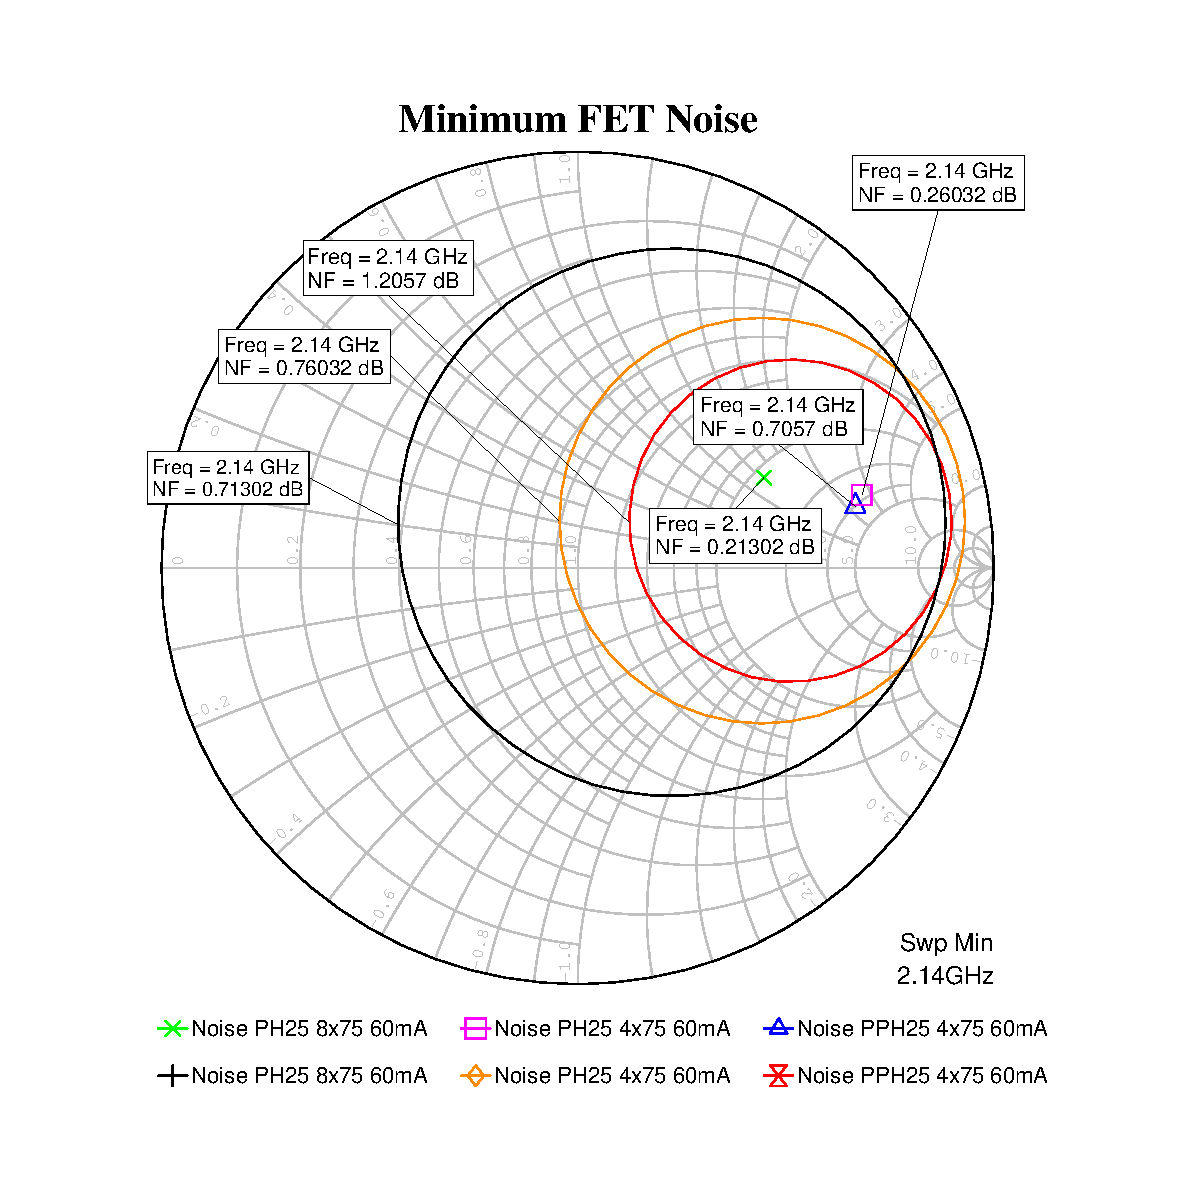
\includegraphics[width=1.0\textwidth]{fig/amplifiers/if1/noisematch}
				\includesmith{0.8\textwidth}{fig/amplifiers/if1/noisematch}
				\caption[$\Gamma_{opt}$ and constant noise circles for UMS FETs.]{$\Gamma_{opt}$ and constant noise circles for different UMS FET, both PH25 and PPH25. Both the absolute noise and the noise increase with mismatch is greater for PPH25. The \unit[8$\times$75]{\mum} is the biggest FET available. It has the lowest inherent noise, the most conveniently placed $\Gamma_{opt}$ and is the most linear device (see \autoref{sec:mixerdevice}).}\label{fig:if1noisematch}
			\end{figure}

			\subsubsection{FET selection and input network}
				Based on the noise properties of the FETs (\autoref{fig:if1noisematch}) and previous work with the PH25 process\autocite{gustavsson07}, the \unit[8$\times$75]{\mum} FET is chosen for the amplifier. Fortunately both low noise and linear operation favours a large device. The input network is a simple L-shaped inductor-inductor impedance matching network.

			\subsubsection{Attenuator}
				The system design requires the amplifier to have a certain gain. If the gain of this amplifier is higher, the total $IIP_3$ will suffer and if it is lower the final noise will increase. As the amplifier's gain is higher than the specified \unit[12]{dB} an attenuator consisting of two resistors is placed at the end. It is designed to optimize the input and output matching as well as add to the stability.\autocite{delpy06} An alternative to an attenuator is parallel feedback (as in IF amplifier 2). This design would however degrade the noise figure and has therefore been discarded.

		\subsection{Schematics and layout}
			The schematic of amplifier IF1 is shown in \autoref{fig:if1schematic}. The corresponding layout is found in \autoref{fig:if1layout}.
			
			\begin{figure}[hbt!]
				\centering
				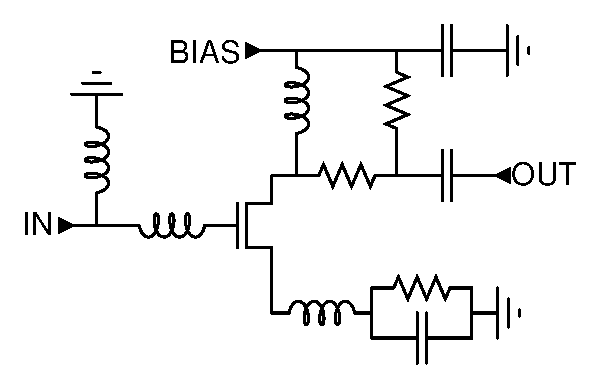
\includegraphics[width=0.7\textwidth]{fig/amplifiers/if1/sch_if1}
				\caption[Amplifier IF1 schematic.]{Schematic of amplifier IF1.}\label{fig:if1schematic}
			\end{figure}

			\begin{figure}[hbt!]
				\centering
				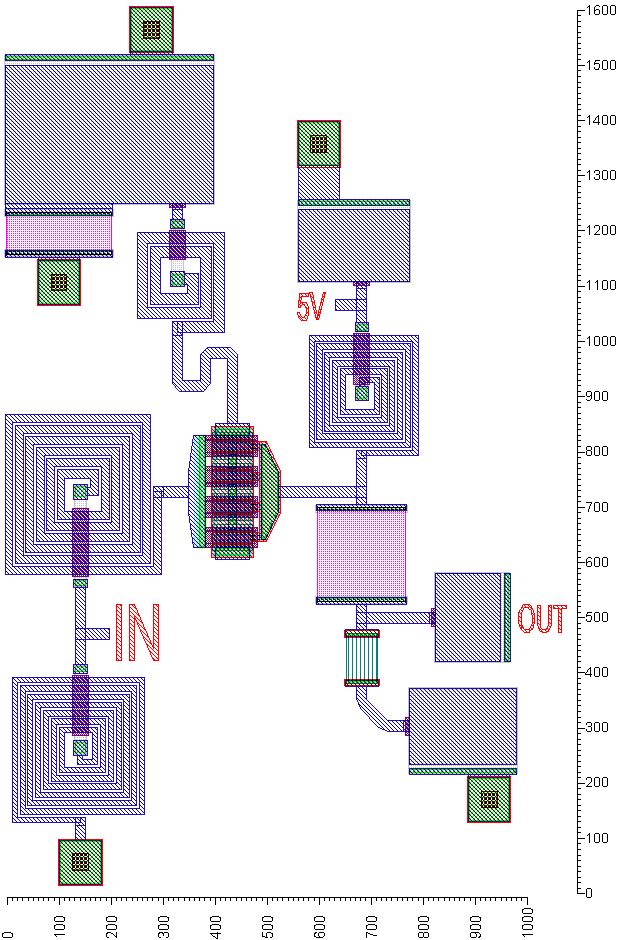
\includegraphics[width=0.7\textwidth]{fig/amplifiers/if1/layout}
				\caption[Amplifier IF1 layout.]{Layout of amplifier IF1.\scalemum}\label{fig:if1layout}
			\end{figure}

		\subsection{Simulation results}
			The simulated performance of amplifier IF1 is found in \autoref{tab:resultif1}. Spread analysis is reported in \autoref{sec:yieldif1} together with plots of the simulation data.  The full spectrum gain is plotted in \autoref{fig:if1gain}.
			
			\begin{table}[hbt!]
				\caption[Simulation results for amplifier IF1.]{Simulation results for amplifier IF1.\disclaimer}
				\label{tab:resultif1}
				\centering
				\begin{tabular}{ l c c c l } \toprule
					Parameter & Min. & Typ. & Max. & Unit \\\midrule
					Frequency range & \multicolumn{3}{c}{2.04--2.24} & GHz \\
					Gain & 11.2 & 11.5 & 11.8 & dB \\
					Return loss input & 12.1 & 14.4 &  & dB \\
					Return loss output & 16.5 & 16.9 &  & dB \\
					Stability $K$@\unit[0--80]{GHz} & >1 & >1 &  &  \\
					$P_{1dB}$ (input) & 5.7 & 6.5 &  & dBm \\
					$IIP_3$ & 19.0 & 19.5 &  & dBm \\
					Power consumption &  & 290 & 290 & mW \\
					Noise figure (estimate) &  & 1.5 & 1.8 & dB \\\bottomrule
				\end{tabular}
			\end{table}
			
			\begin{figure}[hbt!]
				\centering
				\includerect{0.7\textwidth}{fig/amplifiers/if1/widegain}
				\caption[Amplifier IF1 gain.]{Gain of amplifier IF1.}\label{fig:if1gain}
			\end{figure}
		
%		\subsubsection{Source Pull Analysis}
%			A source pull analysis that plots constant noise figure curves along with the optimal $S_{11}$ input match has been conducted (\autoref{fig:if1sourcepull}). The contours show that low noise and good matching overlap fairly good. This is overlap is mostly due to the series feedback.

		\subsection{Discussion}
			The narrowband property of the amplifier enables a design in which parallel feedback can be omitted. This has a good impact on the noise figure but it also gives a steep gain slope and a gate that is hard to match. One consequence is that the matching inductors become very large which in turn increases the noise figure as the UMS inductors have a somewhat low quality factor Q. Another consequence is that would the frequency characteristics shift only \unit[100]{MHz} during fabrication the performance of the amplifier will change dramatically. Detailed frequency dependence can be found in \autoref{sec:yieldif1}.
			
			A noise figure of \unit[1.5]{dB} can by LNA-standards not be considered low. In the PH25 process this value could very well be cut in half.\autocite{kyuko96} Still, amplifier IF1 is not designed only to produce  low  noise, but also to have linear operation. This leads to a compromise in which the power-PH25 process without noise models is used.

%			\begin{figure}[hbt!]
%				\centering
%				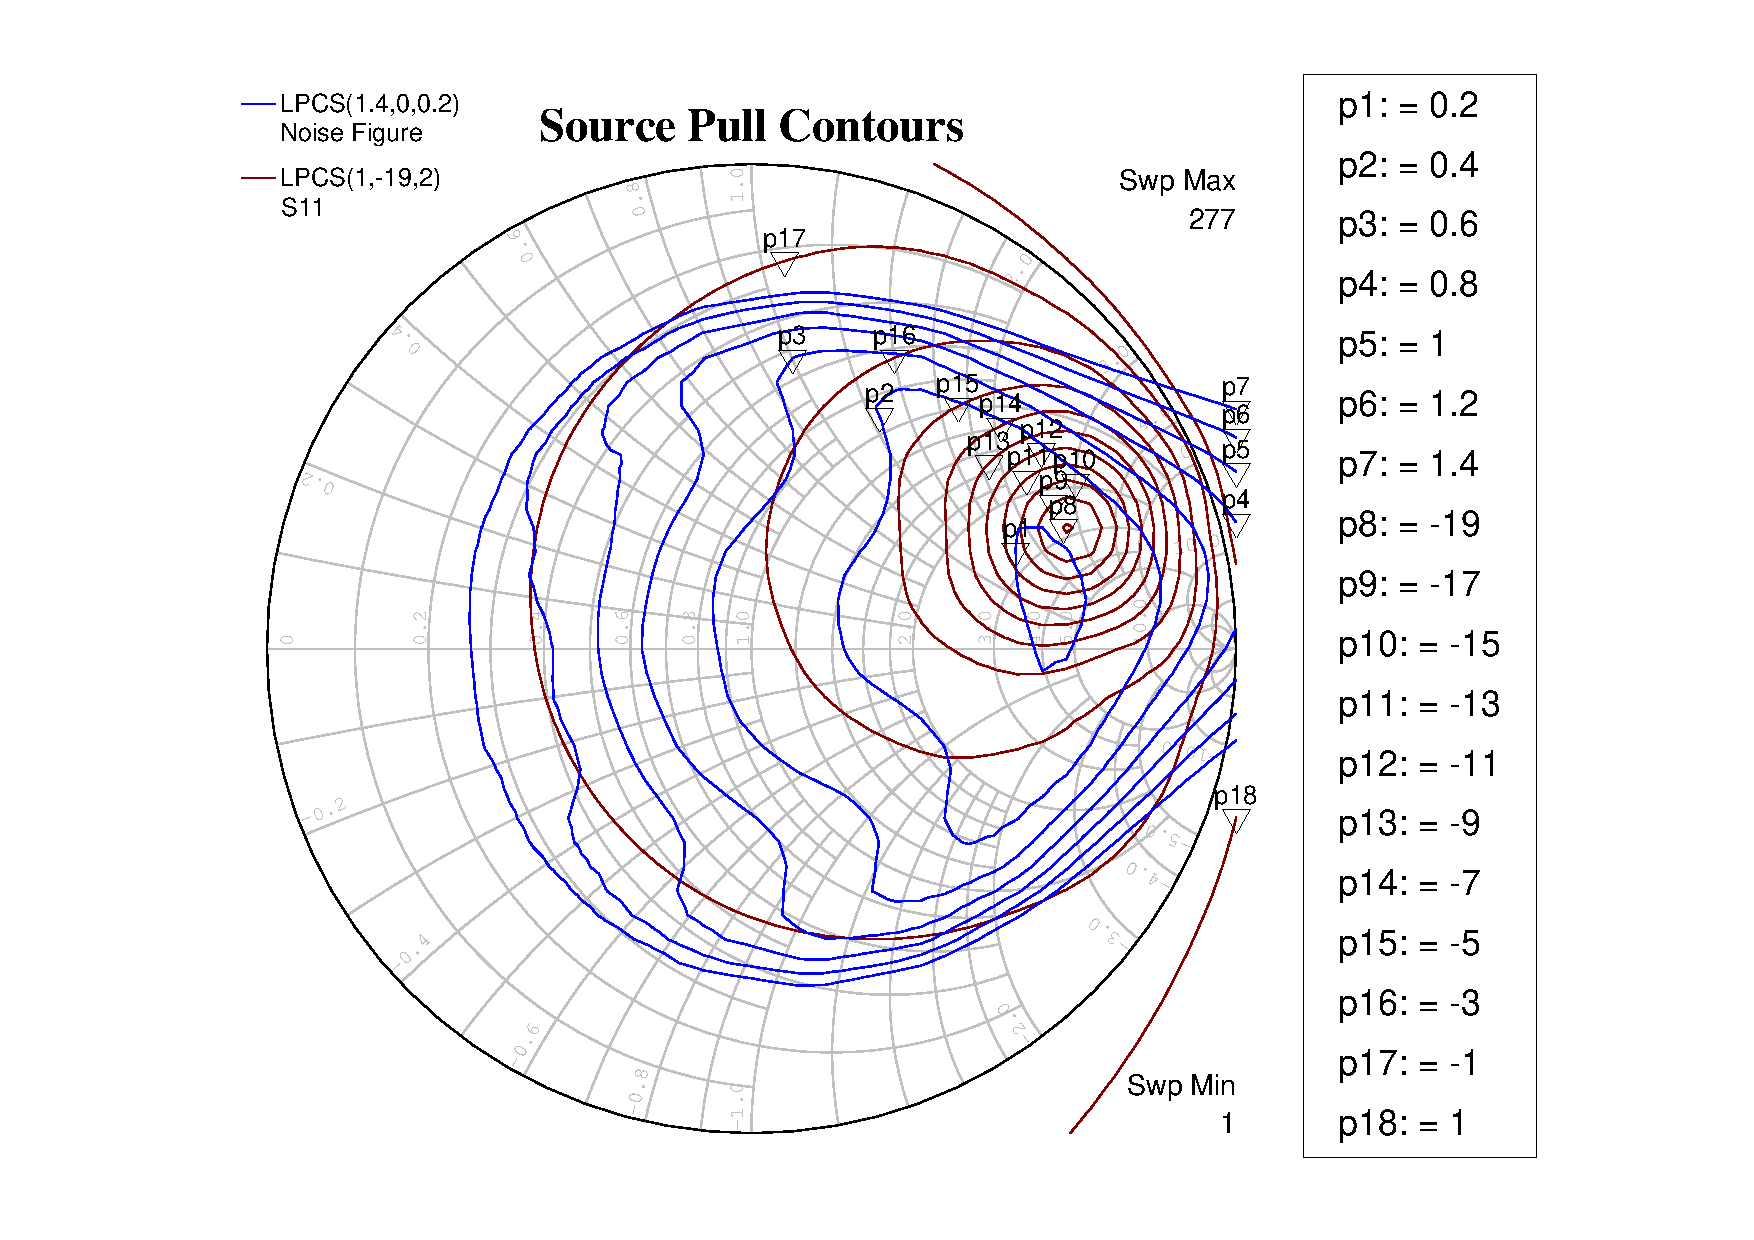
\includegraphics[width=1.0\textwidth]{fig/amplifiers/if1/sourcepull}
%				\caption[Source pull diagram for optimal noise figure.]{Source pull diagram for optimal noise figure and input match. The the optimal points for the two quantities overlap fairly good. The noise value is not that sensitive to the source impedance. The area for which the value stays below \unit[0.4]{dB} is large. It is therefore likely that the noise originating from the components matching the input of the amplifier will cause more noise than mismatching the input itself will.}\label{fig:if1sourcepull}
%			\end{figure}

	\section{High-power IF-amplifier}
		\subsection{Introduction}\label{sec:if2power}
			The last amplification stage has together with the mixing component the biggest impact on the overall chip linearity. As discussed earlier, the more DC-power provided, the more linear the operation becomes. Because the signal has already been amplified once the overall noise figure is not very sensitive to the noise here. High power devices generate a lot of heat and this has to be taken into consideration.

		\subsection{Design}
			\subsubsection{Principle}
				To design a high linearity amplifier a method similar but opposite to the one used to design a LNA is used. Instead of matching the input to the noise optimum the output is matched to peak $P_{1dB}$. The first step is to create a stable and input-matched circuit. Feedback circuits are used to control the gain and the linearity of the amplifier. Using this amplifier load-pull simulations are made for different bias points. This way it's possible to see which bias point and output matching network give the most linear operation.\autocite{anand08}

			\subsubsection{Thermal considerations}
				Calculations performed on the FETs' junction temperatures show that in order to handle the available power and the specified ambient temperature there has to be two FETs. With only one \unit[8$\times$75]{\mum} FET the junction temperature $T_j$ exceeds \unit[170]{$^\circ C$} which is the maximum rating for a GaAs FET. $T_j$ is calculated using thermal resistance models\autocite{fukui80}, where $T_0$ is set to $\unit[100]{^\circ C}$:

				\begin{equation}
					T_j=T_0+P_{FET}R_{TH}
				\end{equation}

				$P_{FET}$ is the power dissipated over the FET and $R_{TH}$ is the FETs thermal resistance according to the models. $T_0$, the temperature on the backside of the chip, is the sum of the ambient temperature and the estimated thermal resistance in the circuit board and the chip package. If the total thermal resistance is $\unit[15]{^\circ C}$, the chip can handle an ambient temperature of $\unit[100]{^\circ C}-\unit[15]{^\circ C}=\unit[85]{^\circ C}$.

				With two \unit[6$\times$75]{\mum} FETs the maximum $T_j$ becomes $\approx$ \unit[150]{$^\circ C$}, which is a high although manageable temperature. Two FETs placed in parallel can be viewed as one big FET with the number of gate fingers equal to the sum of the parts, thus resulting in an equivalent \unit[12$\times$75]{\mum} FET.

			\subsubsection{Feedback and bias}
				The second IF-amplifier is biased in the same manner as the first one, described in \autoref{sec:bias}. This amplifier has both series feedback and parallel negative feedback. Though very small, the inductor on the source creating the series feedback is needed for stability and gain control. The parallel feedback that connects the drain to the source has an attenuating resistance and a capacitance for DC blocking. The purpose of this feedback is to simplify matching and to provide high bandwidth. Although the signal is of a single frequency it is preferable if not both amplifiers' gain are frequency sensitive. The parallel feedback also makes the amplifier less stable.
				
				The FET's decrease in gain slightly as the temperature rises. To compensate for this loss a resistor of GaAs type is chosen for the parallel feedback. This resistor has a positive temperature gradient. This way the decrease in gain is reduced by the smaller feedback.

		\subsection{Schematics and layout}
			The schematic of amplifier IF2 is shown in \autoref{fig:if2schematic}. The corresponding layout is found in \autoref{fig:if2layout}.
			
			\begin{figure}[hbt!]
				\centering
				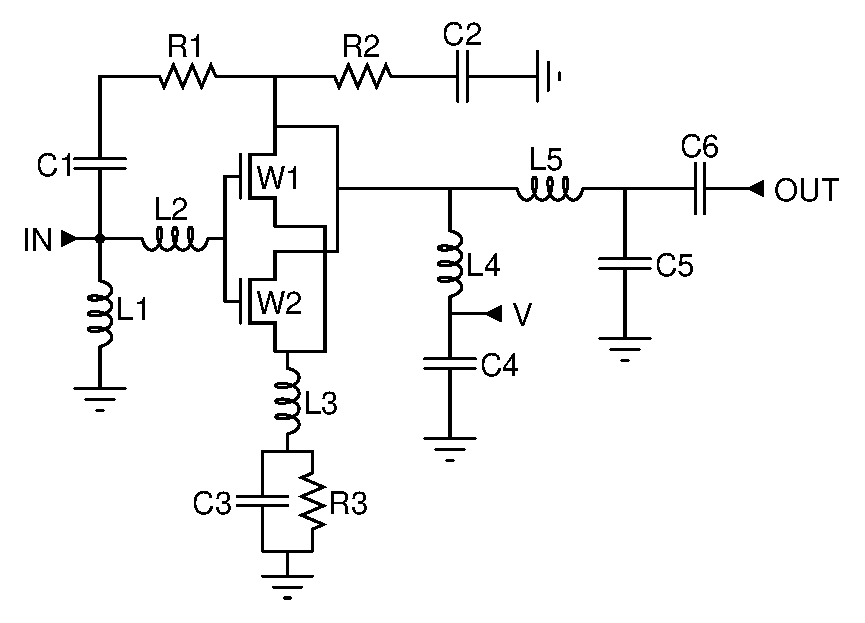
\includegraphics[width=0.75\textwidth]{fig/amplifiers/if2/sch_if2}
				\caption[Amplifier IF2 schematic.]{Schematic of amplifier IF2.}\label{fig:if2schematic}
			\end{figure}

			\begin{figure}[hbt!]
				\centering
				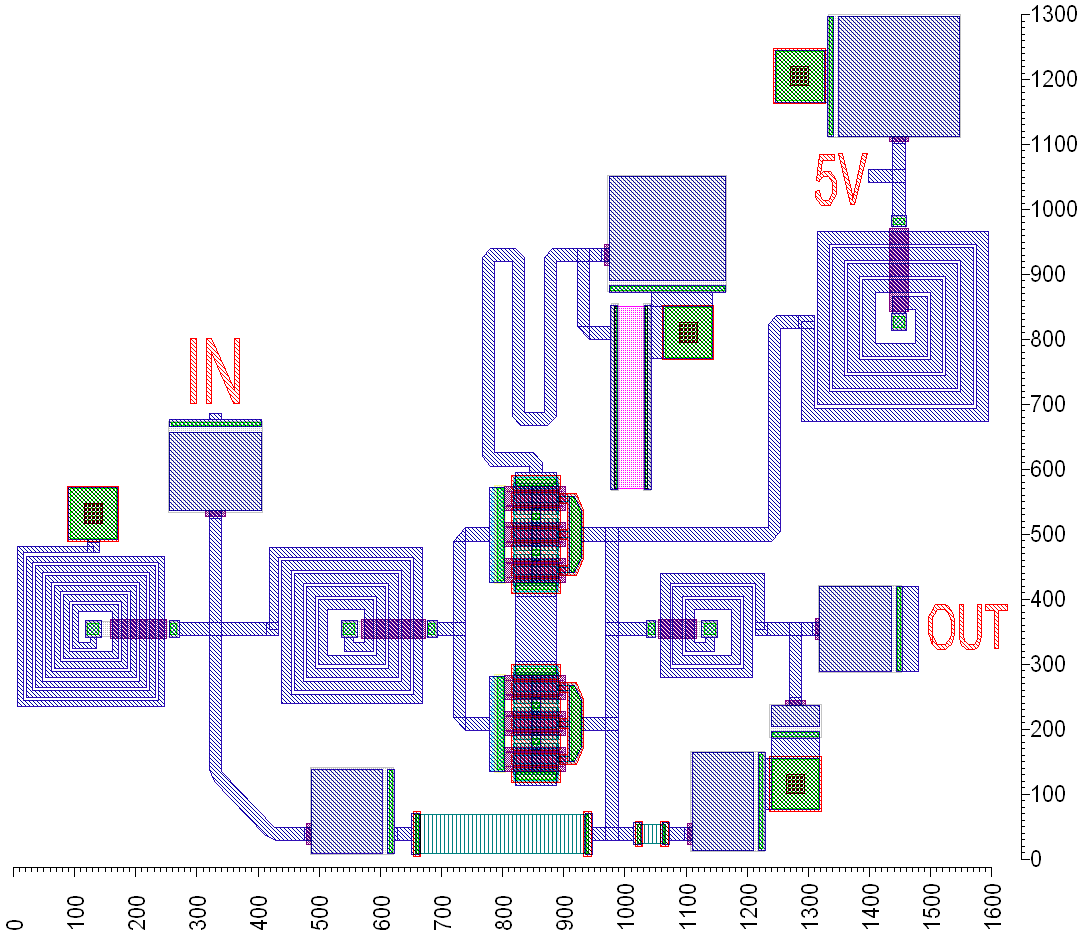
\includegraphics[width=1.0\textwidth]{fig/amplifiers/if2/layout}
				\caption[Amplifier IF2 layout.]{Layout of amplifier IF2.\scalemum}\label{fig:if2layout}
			\end{figure}

		\subsection{Simulation results}
			\subsubsection{Performance overview}
				The simulated performance of amplifier IF2 is found in \autoref{tab:resultif2}. Spread analysis is reported in \autoref{sec:yieldif2} together with plots of the simulation data. The gain is plotted in \autoref{fig:if2gain}.
				
				\begin{table}[hbt!]
					\caption[Simulation results of amplifier IF2.]{Simulation results of amplifier IF2.\disclaimer}
					\label{tab:resultif2}
					\centering
					\begin{tabular}{ l c c c l }\toprule
						Parameter & Min. & Typ. & Max. & Unit \\\midrule
						Frequency range & \multicolumn{3}{c}{2.04--2.24} & GHz \\
						Gain & 12.0 & 12.1 & 12.1 & dB \\
						Return loss input & 24.9 & 25.5 &  & dB \\
						Return loss output & 18.0 & 19.7 &  & dB \\
						Stability $K$@\unit[0--70]{GHz} & >1 & >1 &  &  \\
						$P_{1dB}$ (input) & 10.4 & 10.4 &  & dBm \\
						$IIP_3$ & 22.0 & 22.5 &  & dBm \\
						Power consumption &  & 550 & 550 & mW \\
						Noise figure (estimate) &  & 2.0 & 2.3 & dB \\\bottomrule
					\end{tabular}
				\end{table}
				
				\begin{figure}[hbt!]
					\centering
					\includerect{0.7\textwidth}{fig/amplifiers/if2/widegain}
					\caption[Amplifier IF2 gain.]{Gain of amplifier IF2.}\label{fig:if2gain}
				\end{figure}

			\subsubsection{Linearity analysis}
				The \unit[1]{dB}-compression point, $P_{1dB}$, is simulated for different $i_{ds}$ (\autoref{fig:if2p1dbvspower}). A load pull analysis with both the output matching and $P_{1dB}$ analysed is shown in \autoref{fig:if2lp}. The analysis shows the importance of choosing a correct, and in this case high power, bias point to optimize the two quantities. From the three plots combined it can be seen that the linearity increases dramatically with increased power until peak $P_{1dB}$ is aligned with optimum output match. After that, the increase is only linear. This overall linearity increase agrees with the discussion about power utilisation in the introduction {\autoref{sec:power}}.

				\begin{figure}[h!]
					\centering
					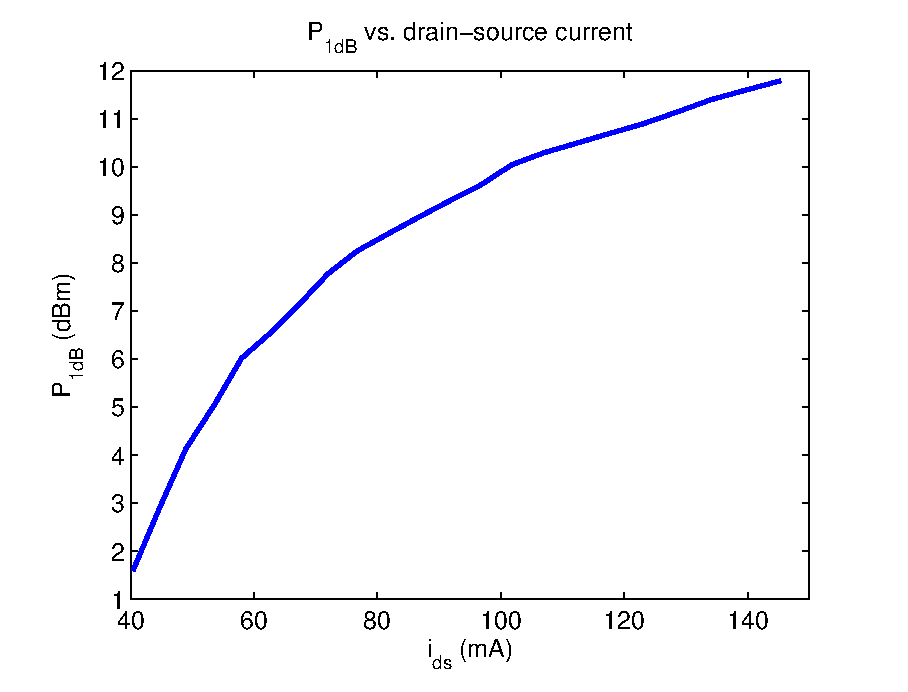
\includegraphics[width=0.7\textwidth]{fig/amplifiers/if2/p1dbvscurrent}
					\caption[Amplifier IF2 $P_{1dB}$ versus $i_{ds}$.]{Amplifier IF2 $P_{1dB}$ versus $i_{ds}$. The increase with increased power is non-linear in the beginning. From approximately \unit[90]{mA} the increase is linear.}\label{fig:if2p1dbvspower}
				\end{figure}				
				
				\begin{figure}[h!]
					\centering 
					\subfloat[][Power consumption 400 mW corresponding to drain-source current 80 mA.]{
						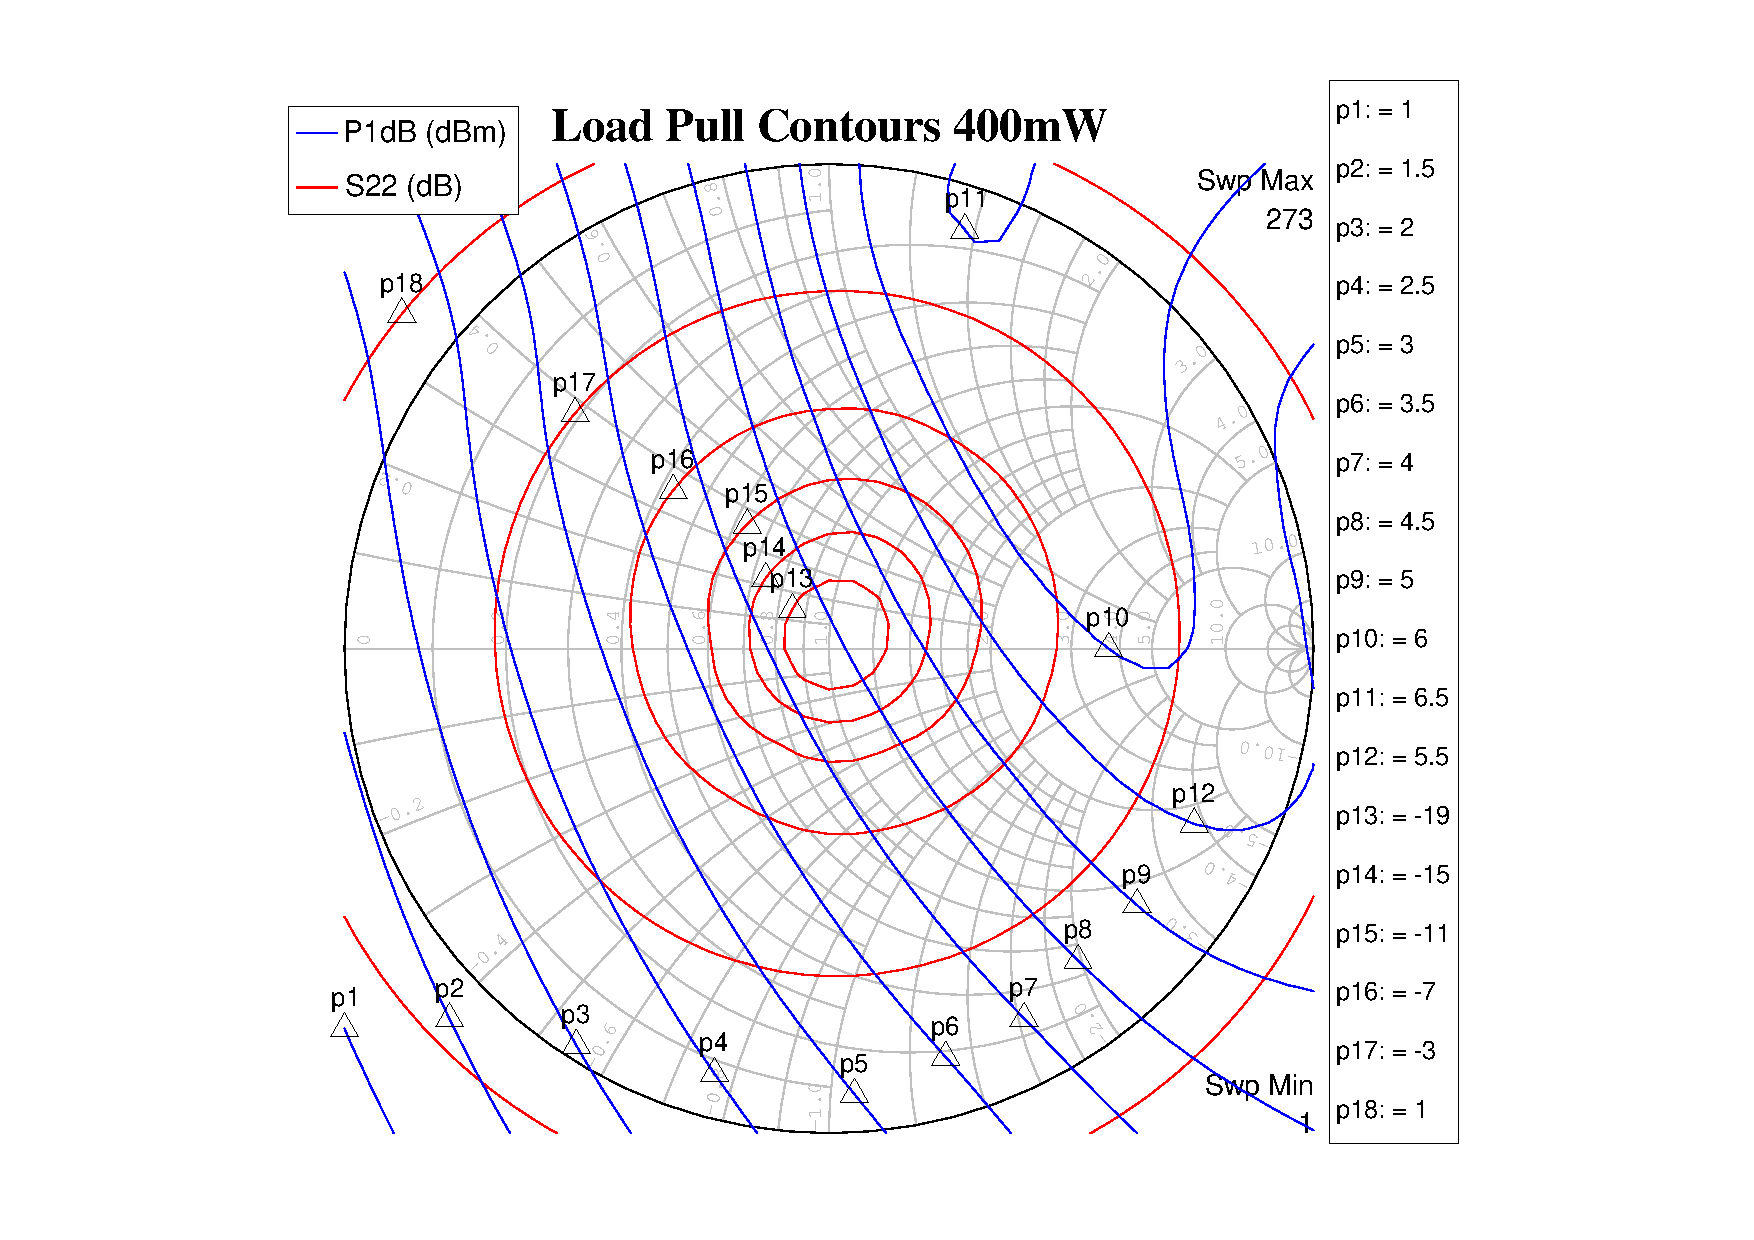
\includegraphics[trim=120 35 125 35, clip, width=0.7\textwidth]{fig/amplifiers/if2/loadpull400}
						\label{fig:if2lp400}
					} \\
					\subfloat[][Power consumption 550 mW corresponding to drain-source current 110 mA.]{
						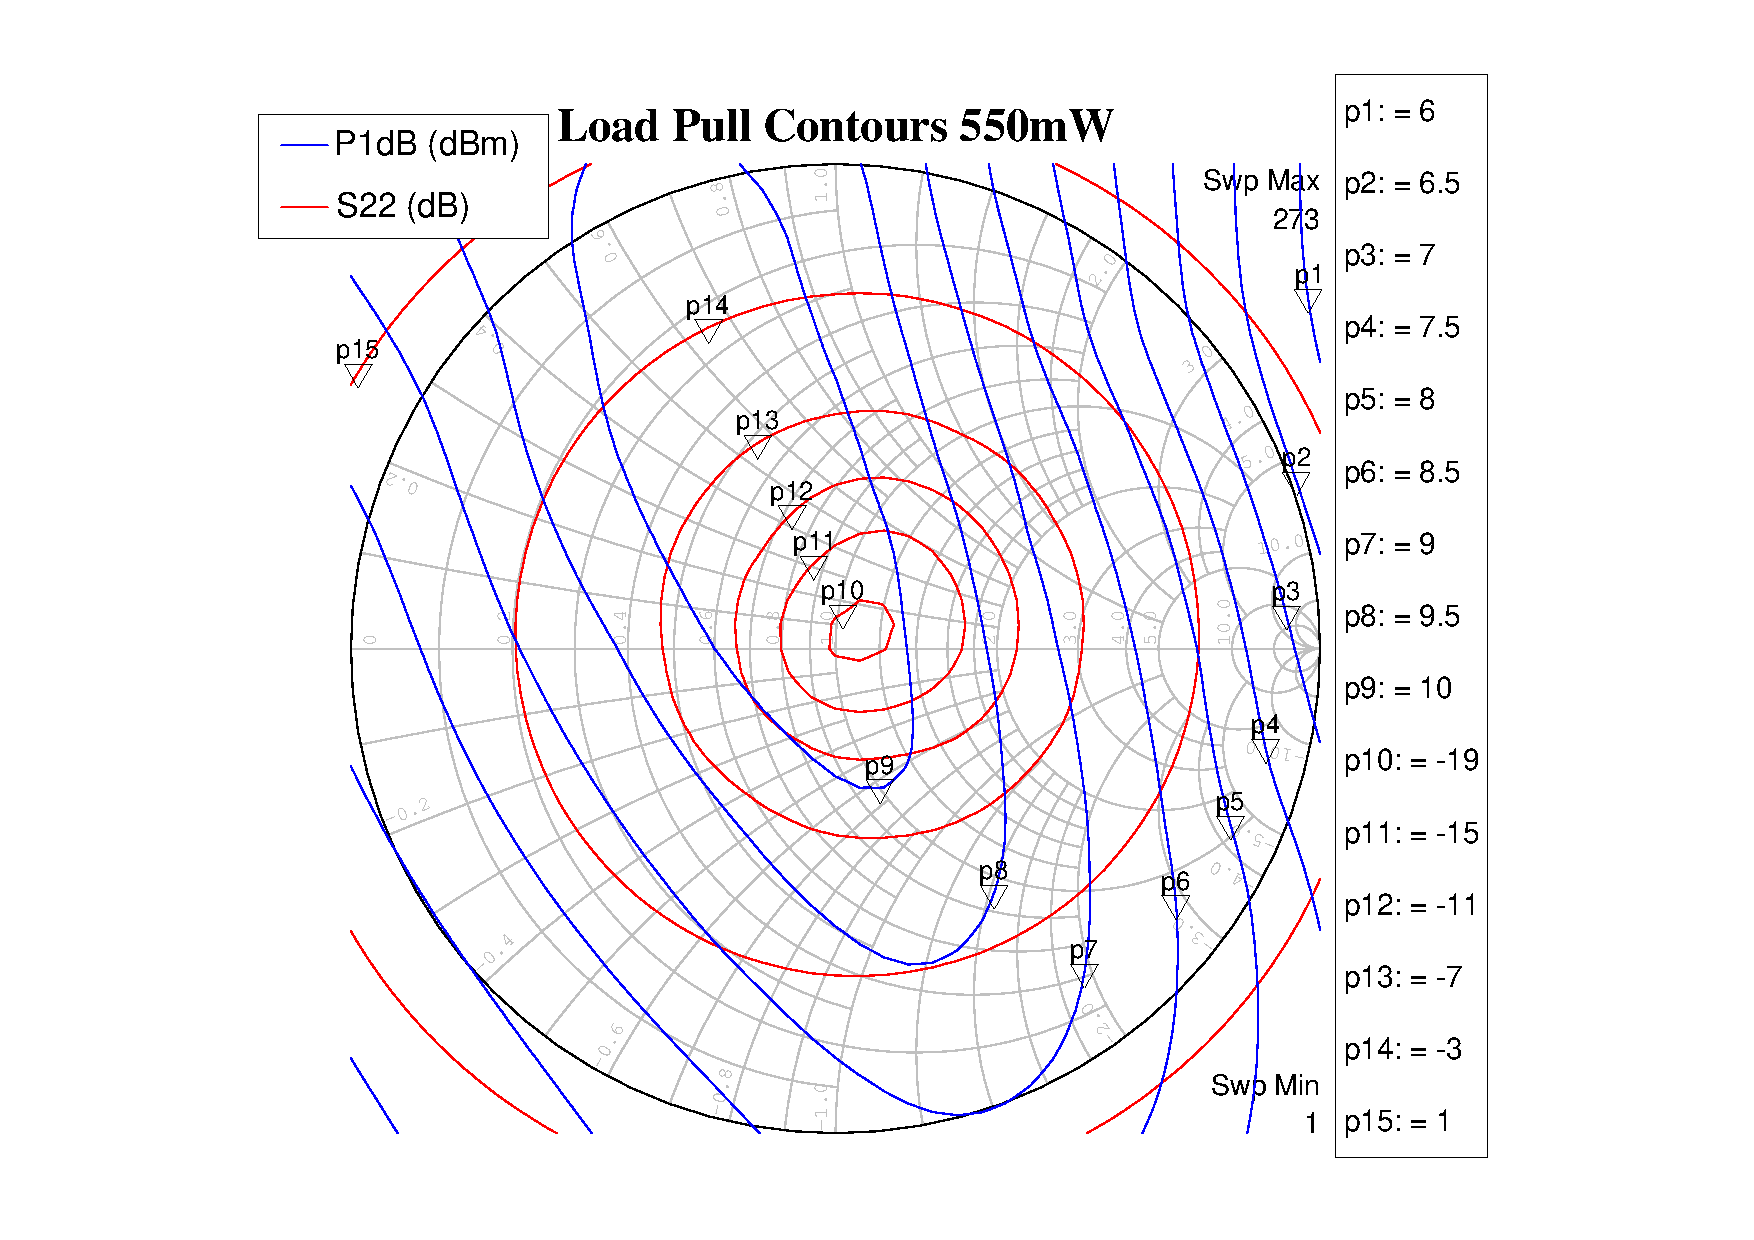
\includegraphics[trim=120 35 125 35, clip, width=0.7\textwidth]{fig/amplifiers/if2/loadpull550}
						\label{fig:if2lp550}
					} 
					\caption[Load pull diagrams for IF amplifier 2.]{Load pull diagrams for optimal linearity (deformed contours) and optimal output matching (circular contours). The analysis is applied to a stable and matched amplifier with two \unit[6$\times$75]{\mum} FETs. The load pull diagrams show that devices biased in the most linear and high power region of the iv-curve (point C in \autoref{fig:fet_bias_point}) not only give a higher \unit[1]{dB} compression point overall but also a better match of the maximum $P_{1dB}$ with the optimal output impedance match.}\label{fig:if2lp}
				\end{figure}
				
		\subsection{Discussion}
			The thermal limitations forced a two-FET amplifier design. This requires more space but effectively splits the source-drain current for each device in half. Another interesting observation is that the amplifier's linearity increased in the process. $P_{1dB}$ increased with \unit[4]{dBm} keeping the power consumption unchanged. The reason for this increase is attributed the same general reason why large devices are preferred over small when designing high-linearity class A amplifiers.
			
			Even though the junction temperature in the FETs has been reduced dramatically with the dual-FET design, the asymmetric design with only one source network causes a large current to flow through the upper transistor. The FET connected to the source has the DC-current of the other transistor in the source. In these UMS FETs the source layers are connected with \unit[14]{\mum} air bridges. According to the maximum ratings these layers can only handle \unit[7.5]{mA/\mum}. This gives a total of $\unit[105]{mA}$ and the design is just above that ($\unit[110]{mA}$). The three alternatives are either to reduce the current $\unit[5]{mA}$, to widen the air bridge \unit[1]{\mum} or to route a common source for both FETs from the middle strip via an air bridge.
			
			The implemented negative parallel feedback provides wider bandwidth and easier matching. The bandwidth may seem unnecessary considering the single frequency operation. However, as amplifier IF1 is designed with a steep gain slope it is preferable that this amplifier is not. This is due to the possibility of process variation in the frequency dependence. A variation within the current design limits most damage in performance to amplifier IF1.
			
			The noise figure in the amplifier is approximately \unit[0.5]{dB} higher than in amplifier IF1. This shows that even though the input network is simpler, the parallel feedback will result in an increase in noise. Also, no effort has been made to match noise optimum with the input match in this amplifier.
		
		
		